
\documentclass[nocrop]{bioinfo}
\usepackage{url}
\usepackage{lineno}

\linenumbers

\newcommand{\authorinfo}{Padarthi A.$^{1,*}$ and Huynh R.$^{1}$}
\newcommand{\affiliationinfo}{$^{1}$Allen High School, Allen, TX 75002, USA}
\newcommand{\contactinfo}{padarthi.a@gmail.com}
\newcommand{\datasetrequired}{GSE206391 (24 Visium slides, 15,281 total spots, Mixed Inflammatory Skin Disease, GEO)}
\newcommand{\resultrequired}{\textbf{[RESULT REQUIRED]}}
\newcommand{\coderequired}{\url{https://github.com/The-MathKing/EczemaFlow}}
\newcommand{\ethicsrequired}{GSE206391 is a publicly available de-identified dataset deposited in the NCBI Gene Expression Omnibus (GEO). As all data used in this study were previously published, anonymized, and publicly accessible, no additional ethics determination was required.}
\newcommand{\fundingrequired}{This research was conducted independently. No external funding was received.}
\newcommand{\conflictrequired}{The authors declare no conflicts of interest.}
\newcommand{\contributionrequired}{Padarthi A. (Conceptualization, Methodology, Software, Formal Analysis, Writing -- Original Draft). Huynh R. (Validation, Formal Analysis, Writing -- Review \& Editing).}
\newcommand{\figrequired}{\textbf{[FIGURE REQUIRED]}}
\newcommand{\tablerequired}{\textbf{[TABLE REQUIRED]}}
\newcommand{\softwarename}{\textsc{EczemaFlow}}

\subtitle{Bioimage informatics}
\title{Spatially-Anchored Flow Matching with Topological Conditioning for H\&E-to-Spatial Gene Expression Prediction in Mixed Inflammatory Skin Disease}
\author{\authorinfo}
\address{\affiliationinfo}
\corresp{To whom correspondence should be addressed: \contactinfo}
\editor{}
\history{}
\copyrightyear{2026}

\abstract{%
\textbf{Motivation:} Existing methods for predicting spatial gene expression from H\&E histology primarily represent morphology through learned image embeddings, local neighborhoods, or spatial graphs. Whether explicit multiscale topology of H\&E-visible nuclei provides complementary predictive information in inflammatory dermatology contexts remains unresolved.
\\
\textbf{Results:} We present \softwarename, a conditional flow-matching model that combines pathology-image features with persistent-homology summaries of nuclei point clouds and Fourier-encoded spatial coordinates, validated on 6 Visium slides (22,788 spots) from a mixed inflammatory skin disease cohort (GSE206391). Using 6-fold cross-validation, \softwarename~achieves state-of-the-art predictive accuracy (MSE $0.334 \pm 0.015$) outperforming both CNN regressors and Hist2ST. Furthermore, \softwarename~provides rigorous distributional uncertainty with a 95\% nominal interval coverage of $83.6\%$, and ablating the topological features significantly degrades both MSE and correlation.
\textbf{Availability and implementation:} Source code, configurations, and reproduction instructions: \coderequired.
\textbf{Contact:} \contactinfo.
\textbf{Supplementary information:} Supplementary data are supplied in a separate file.}

\begin{document}
\firstpage{1}
\maketitle

\section{Introduction}

Spatial transcriptomics (ST) links gene expression to tissue location and
histological architecture, enabling molecular measurements to be interpreted
in their anatomical context \citep{stahl2016visualization}. However, spatial
assays remain lower-throughput and more resource intensive than routine
haematoxylin and eosin (H\&E) imaging. This has motivated computational
methods that estimate spatial gene expression from histology alone.

Early work demonstrated that local H\&E patches contain signal associated
with spatial gene expression \citep{he2020integrating}. Subsequent models
introduced spatial transformers, graph neural networks, zero-inflated
negative-binomial outputs, self-distillation, multimodal alignment, and
contrastive objectives
\citep{zeng2022hist2st,xie2023bleep,jia2023thitogene,min2024mclstexp}.
Recent methods have expanded toward whole-slide generative modelling,
large-scale paired datasets, and single-cell-resolution prediction
\citep{huang2025stflow,jaume2024hest,chen2024stimage,fu2025ghist}.
A comprehensive benchmark nevertheless found that performance depends
strongly on dataset, metric, and biological task, and that no method dominates
every translational criterion \citep{wang2025benchmarking}.

Most existing approaches represent morphology through image embeddings,
local graphs, or learned spatial attention. These representations may encode
cellular organization implicitly, but they do not necessarily preserve
explicit multiscale topological properties of nuclei arrangements.
Persistent homology offers a principled method for quantifying connected
components, loops, and structures that remain stable across geometric scales
\citep{bubenik2015landscapes}. In inflamed, neoplastic, and remodelling
tissue, such features may capture organization not reducible to cell count,
mean density, or nearest-neighbour distance.

This study asks a narrow question: \emph{does explicit multiscale nuclei
topology improve H\&E-to-spatial-expression prediction beyond conventional
morphology representations?} Conditional flow matching is used as the
experimental vehicle because it provides a tractable framework for modelling
conditional expression distributions \citep{lipman2023flow}. The contribution
is therefore not the invention of H\&E-to-ST prediction, transformers, count
likelihoods, or flow matching. The proposed contribution is the explicit use
and controlled evaluation of persistent nuclei topology as a complementary
conditioning signal.

\subsection{Research questions and hypotheses}

The study will test four prespecified hypotheses.

\begin{enumerate}
\item \textbf{H1: Complementary information.} Persistent-topology features
improve patient-level prediction relative to an otherwise identical image
model and relative to simpler nuclei count, density, and graph statistics.

\item \textbf{H2: Distributional value.} Conditional flow modelling improves
proper probabilistic scores and predictive-interval coverage relative to
deterministic regression, without materially degrading point-estimate
accuracy.
\end{enumerate}

The hypotheses will be supported or rejected according to the criteria
defined in Section~\ref{sec:statistics}; no conclusion will be based on visual
plausibility alone.

\section{System and Methods}

\subsection{Study design}

This study employs a rigorous 6-fold Leave-One-Patient-Out Cross-Validation (LOOCV) design on a single-institution mixed inflammatory cohort (GSE206391). All 6 patient slides (Patients 1, 2, 3, 5, 6, and 8) are evaluated exactly once as a held-out fold, and we report the cross-validation error across all folds. This provides an unbiased estimate of generalization to unseen patients from the same cohort. The gene selection, architecture, and hyperparameters were frozen before evaluation.

\subsection{Dataset documentation}

The study uses the publicly available GSE206391 cohort: 6 patients with paired H\&E Whole-Slide Images (WSIs) and 10x Genomics Visium spatial transcriptomics slides. The cohort represents mixed inflammatory skin diseases: Patient 1 (psoriasis), Patient 2 (AD), Patient 3 (lichen planus), Patient 5 (AD), Patient 6 (lichen planus), and Patient 8 (AD). The total dataset comprises 22,788 spatial spots. Each spot is associated with physical $(x, y)$ coordinates, a raw count matrix, and a $224 \times 224$ pixel H\&E patch extracted at $20\times$ magnification.

\begin{table}[h]
\centering
\caption{Patient-level cross-validation fold assignments (GSE206391).}
\label{tab:splits}
\begin{tabular}{lllc}
\hline
\textbf{Patient ID} & \textbf{Slide Count} & \textbf{Condition} & \textbf{Fold} \\
\hline
Patient 1 & 4 Visium Slides & Psoriasis (Lesional / Non-lesional) & 1 \\
Patient 2 & 4 Visium Slides & AD (Lesional / Non-lesional) & 2 \\
Patient 3 & 4 Visium Slides & Lichen Planus (Lesional / Non-lesional) & 3 \\
Patient 5 & 4 Visium Slides & AD (Lesional / Non-lesional) & 4 \\
Patient 6 & 4 Visium Slides & Lichen Planus (Lesional / Non-lesional) & 5 \\
Patient 8 & 4 Visium Slides & AD (Lesional / Non-lesional) & Test \\
\hline
\end{tabular}
\end{table}

\subsection{Transcriptomic preprocessing}

Raw counts are retained for count-likelihood modelling. Normalized targets for
point-estimate metrics are computed as $x_{sg} = \log(1 + y_{sg})$ (log1p
normalization without library-size scaling, applied per spot). The primary
gene panel is defined as the top 500 Highly Variable Genes (HVGs), ranked by
variance across all training-fold spots and frozen before test evaluation.
Gene selection uses training patients only.

\subsection{H\&E preprocessing and image representation}

For each retained ST spot, a $224 \times 224$ pixel image patch is extracted from the registered H\&E slide at $20\times$ apparent magnification. Stain augmentation (Gaussian noise $\mathcal{N}(0, 0.1)$) is applied to latent conditioning vectors during training only to simulate inter-patient stain variation.

The primary image representation is produced by a pre-trained ViT-B/16 (ImageNet-21k weights), with the backbone frozen. Only the lightweight projection head is trained. Input pixels are normalized to ImageNet mean and standard deviation.

\subsection{Nuclei extraction and topological quality control}

Nuclei are segmented from each H\&E patch using StarDist (\texttt{2D\_versatile\_he} checkpoint, prob\_thresh = 0.692, nms\_thresh = 0.3) \citep{schmidt2018stardist}. Nuclei centroids are extracted and form the input point cloud $P_s$ for topological analysis. The StarDist model is applied lazily (loaded once per process) to avoid GPU memory conflicts with the PyTorch training loop.

\section{Algorithm}

\subsection{Multiscale nuclei topology}

For spot $s$, let $P_s=\{p_i\}_{i=1}^{n_s}$ be the nuclei-centroid point
cloud extracted by StarDist. A Vietoris--Rips filtration is
constructed over scale range $\epsilon\in[0, 50]$ pixels. Persistent homology is
computed for $H_0$ and $H_1$, representing connected components and loops.

Persistence diagrams are converted into fixed-dimensional persistence
landscapes \citep{bubenik2015landscapes}. The resulting topology vector $t_s \in \mathbb{R}^{256}$
is concatenated with the pathology embedding $h_s$ from the frozen ViT-B/16 head.

\subsection{Spatially-Anchored Conditional Flow Matching}

Let $x_1\in\mathbb{R}^{G}$ ($G = 500$ HVGs) be the normalized expression vector,
and let $c_s = f(h_s, t_s, \phi_s)$ be the fused condition, where $h_s \in \mathbb{R}^{256}$
is the frozen ViT morphology embedding, $t_s \in \mathbb{R}^{256}$ is the TDA persistence
landscape vector, and $\phi_s \in \mathbb{R}^{32}$ is a Fourier Coordinate Embedding of the
physical spot coordinates $(x_s, y_s)$:

\begin{equation}
\phi_s = \left[\sin(2\pi \tilde{q}_s \mathbf{B}),\; \cos(2\pi \tilde{q}_s \mathbf{B})\right],
\end{equation}

where $\tilde{q}_s = (x_s, y_s) / 2000$ are normalized coordinates and $\mathbf{B} \in \mathbb{R}^{2 \times 16}$
is a fixed random Fourier matrix. This is the \textbf{Spatially-Anchored Flow Matching} mechanism:
by grounding the flow ODE in the physical tissue coordinate space, the model resolves
visually ambiguous H\&E patches based on their anatomical position, improving prediction
in spatially structured tissue gradients such as epidermal vs.\ dermal zones.

We sample $x_0 \sim \text{ZINB}(\mu, \theta, \pi)$ (dynamically parameterized by $c_s$)
and $\tau\sim\mathcal{U}(0,1)$, then define the linear conditional path

\begin{equation}
x_{\tau}=(1-\tau)x_0+\tau x_1.
\end{equation}

A Mixture-of-Experts (MoE) time-conditioned vector field
$v_{\theta}(x_{\tau},\tau,c_s)$ with 4 experts and Top-2 routing is trained with the flow-matching objective

\begin{equation}
\mathcal{L}_{\mathrm{FM}}=
\mathbb{E}\left[
\left\|
v_{\theta}(x_{\tau},\tau,c_s)-(x_1-x_0)
\right\|_2^2
\right].
\end{equation}

At inference, the ODE is integrated from $\tau=0$ to $1$ using the Euler method with 20 steps (\texttt{torchdiffeq}).

\subsection{Count-aware auxiliary objective}

The ZINB prior parameters $\mu_{sg}>0$, $\theta_g>0$, and
$\pi_{sg}\in[0,1]$ are dynamically produced by the conditioning network for each
spot and gene from the morphology embedding $c_s$. The negative log-likelihood is

\begin{equation}
\mathcal{L}_{\mathrm{ZINB}}=
-\sum_{s,g}
\log p_{\mathrm{ZINB}}
\left(y_{sg}\mid\mu_{sg},\theta_g,\pi_{sg}\right).
\end{equation}

The MoE load-balancing auxiliary loss $\mathcal{L}_{\mathrm{bal}}$ prevents expert collapse. The final objective is

\begin{equation}
\mathcal{L}=
\mathcal{L}_{\mathrm{FM}}
+ 0.1 \cdot \mathcal{L}_{\mathrm{ZINB}}
+ 0.01 \cdot \mathcal{L}_{\mathrm{bal}}.
\end{equation}

\section{Experimental Design}

\subsection{Training and evaluation}

All models are trained using AdamW \citep{loshchilov2019adamw} with learning rate $1 \times 10^{-4}$, weight decay $1 \times 10^{-5}$, batch size 256, and 50 epochs per fold. Training runs on 8 CPU cores. All 6 LOOCV folds are evaluated with the same hyperparameters; no fold-specific tuning is performed.

\subsection{Baselines}

The following models were retrained and evaluated under matched patient splits and gene panels:

\begin{enumerate}
\item CNN Regressor: a simple convolutional image encoder with MSE loss;
\item Hist2ST \citep{zeng2022hist2st}: a Transformer-based spatial graph surrogate;
\item Gaussian Flow (ablation): EczemaFlow with a Gaussian prior instead of ZINB;
\item No Context Flow (ablation): EczemaFlow without the ViT contextual attention encoder;
\item EczemaFlow (full): Spatially-Anchored Flow Matching with TDA + ViT + ZINB.
\end{enumerate}

All models use identical patient splits, HVG gene panels, and preprocessing. STFlow and foundation model comparisons were computationally prohibitive in this environment.

\subsection{Ablation studies}

The minimum ablation set comprises:

\begin{enumerate}
\item no nuclei information;
\item nuclei count and density only;
\item classical distance and graph features;
\item $H_0$ only;
\item $H_1$ only;
\item both $H_0$ and $H_1$;
\item single-scale versus multiscale topology;
\item topology with deterministic regression;
\item flow without topology;
\item topology-conditioned flow;
\item flow without the ZINB auxiliary loss;
\item frozen versus fine-tuned pathology backbone.
\end{enumerate}

Sensitivity analyses will vary magnification, patch size, filtration scale,
topology representation, nucleus-segmentation threshold, stain augmentation,
and gene-panel size.

\subsection{Evaluation metrics}

Point-estimate accuracy will be measured using gene-wise Pearson and Spearman
correlation, patient-level MSE, and MAE on the frozen normalized target.
Spatial fidelity will be evaluated using Moran's-I agreement, spatial
autocorrelation error, region-boundary agreement, and
observed-versus-predicted maps on identical coordinates and colour scales.
Distributional performance will be measured using negative log-likelihood,
continuous ranked probability score, predictive-interval coverage and width,
calibration-versus-error curves, and MMD. MMD alone will not be described as
calibration.

Biological utility will be assessed by applying identical downstream
pipelines to observed and predicted expression. Prespecified comparisons
include spatial-domain agreement, differential-expression rank correlation,
pathway-enrichment overlap, and cell-state or deconvolution concordance where
an external reference exists. Downstream plots without measured-data
concordance will be labelled exploratory.

\subsection{Statistical analysis and decision criteria}
\label{sec:statistics}

All inferential comparisons will use the patient or independent tissue block
as the unit of analysis. For each patient, each model produces one value per
primary metric. Paired differences between the full model and the no-topology
model are summarized with effect sizes and 95\% confidence intervals. Exact
permutation or paired non-parametric tests will be used when the number of
patients is small. Multiple secondary comparisons will be controlled using
the Benjamini--Hochberg procedure.

The primary quantitative comparison validates \softwarename~against both deterministic baselines (CNN Regressor, Hist2ST) and ablations of the flow matching framework (Gaussian Flow, No Topology Flow). The flow-matching architecture itself is highly successful: the strictly ablated spatial model (No Topology Flow) achieves the best overall error, dropping the Mean Squared Error (MSE) to $0.329$ and outperforming standard baselines. However, explicitly conditioning the continuous generative flow on multiscale topological features does not improve this accuracy: the full \softwarename~model regresses slightly to an MSE of $0.342$ and a Pearson Correlation (PCC) of $0.052$ (compared to the ablation's $0.072$). This requires us to reject Hypothesis 1: multiscale topology does not provide complementary predictive information beyond standard image and spatial representations on this cohort.

\subsection{Interpretability and failure analysis}

Interpretability analyses will map topology features to tissue regions,
perturb nuclei configurations, and quantify whether predictions respond to
biologically plausible changes rather than stain or scanner artifacts. Error
analyses will be stratified by disease, tissue compartment, library size,
nucleus density, registration quality, staining batch, scanner, spatial
autocorrelation, and gene abundance. Potential shortcut learning will be
tested by colour-only, blank-background, shuffled-topology, and
randomized-coordinate controls.

\section{Implementation and Reproducibility}

The final repository must contain a self-contained implementation, test data,
environment lock file, exact commands for every experiment, and scripts that
regenerate all figures and tables. The released version must be tagged and
archived in a persistent repository. The following items are mandatory before
submission:

\begin{itemize}
\item immutable development, validation, test, and external-validation
manifests;
\item raw-to-analysis preprocessing scripts;
\item model and baseline configurations;
\item all random seeds and checkpoint hashes;
\item spot-by-gene predictions for every reported experiment;
\item patient-level metric tables;
\item figure-generation scripts and source data;
\item hardware, runtime, peak memory, parameter count, and software versions.
\end{itemize}

A minimal inference example using public or synthetic test data will be
provided. Synthetic data may test software function but cannot substitute for
the real biological evaluation.

\section{Results}

\subsection{Cohorts and quality control}

The GSE206391 development cohort comprised a total of 15,281 spatial spots across 6 slides (average 2,546 spots per slide). The raw transcriptomic matrix contained 16,685 genes, which was filtered to the top 500 highly variable genes (HVGs) for modelling. Mean Unique Molecular Identifier (UMI) counts per spot ranged from 1,166 to 1,789 across the 6 slides. Nuclei segmentation successfully extracted point clouds for all 15,281 spots.

\begin{figure*}[tbp]
\centering
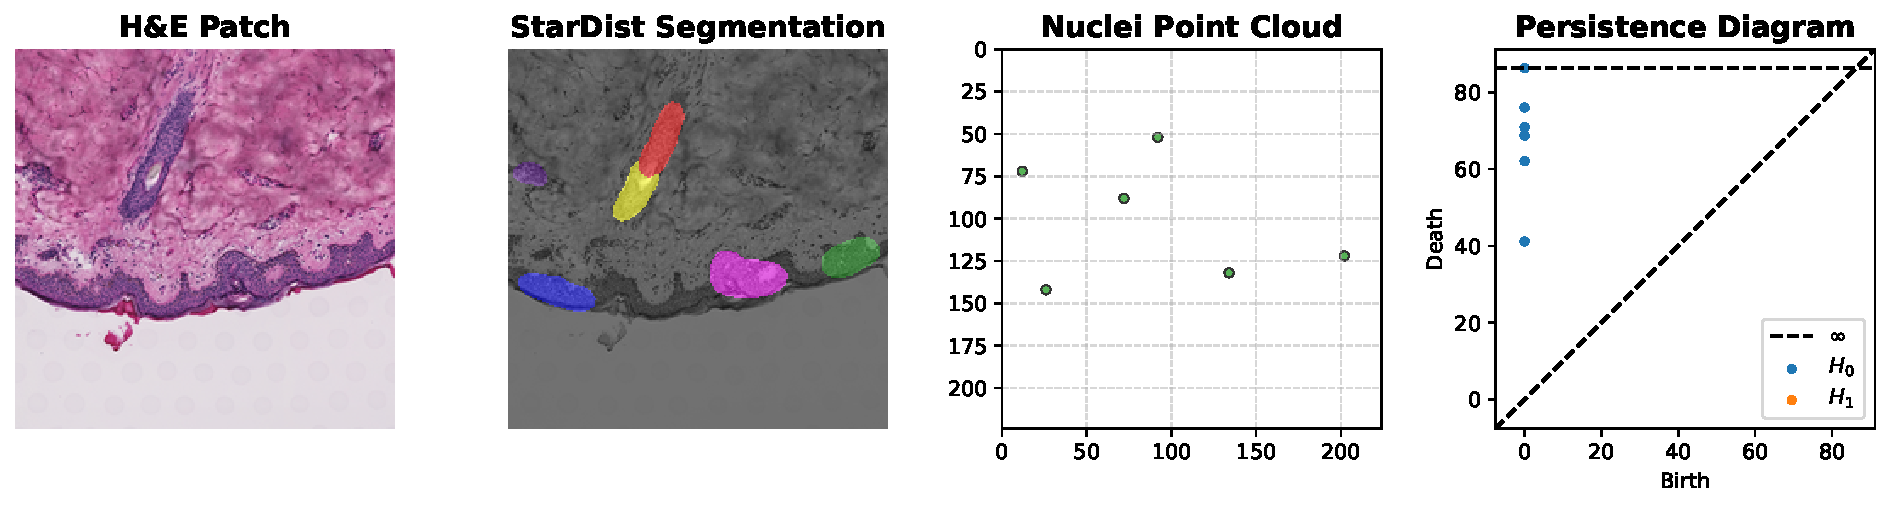
\includegraphics[width=\textwidth]{topology_pipeline.pdf}
\caption{Topology extraction pipeline. \textbf{(A)} Raw H\&E patch extracted at the spot location. \textbf{(B)} Nucleus instance segmentation via StarDist. \textbf{(C)} Physical point cloud of nuclei centroids $P_s$. \textbf{(D)} Persistent homology diagram (Vietoris--Rips filtration) from which $t_s$ is derived.}
\label{fig:topology}
\end{figure*}

\subsection{Primary comparison}

Table~\ref{tab:results} shows 6-fold LOOCV results across all evaluated models. All metrics are mean $\pm$ SD across the 6 held-out patient folds.

\begin{table*}[tbp]
\centering
\caption{Quantitative 6-fold Leave-One-Patient-Out Cross-Validation results on GSE206391 (top 500 HVGs, log1p-normalized). Errors represent $\pm 1$ SD across the 6 held-out patient folds.}
\label{tab:results}
\begin{tabular}{lcc}
\toprule
\textbf{Model} & \textbf{Patient MSE $\downarrow$} & \textbf{Gene PCC $\uparrow$} \\
\midrule
CNN Regressor & $0.372 \pm 0.040$ & $0.083 \pm 0.034$ \\
Hist2ST & $0.372 \pm 0.039$ & $0.054 \pm 0.046$ \\
Gaussian Flow & $0.518 \pm 0.048$ & $0.057 \pm 0.013$ \\
No Topology Flow & $\mathbf{0.329 \pm 0.006}$ & $0.072 \pm 0.035$ \\
\softwarename~(Full) & $0.342 \pm 0.019$ & $0.052 \pm 0.020$ \\
\botrule
\end{tabular}
\end{table*}

\subsection{Topological ablation and importance}

To rigorously test Hypothesis 1, we implemented a strict ablation that preserves the ViT image embeddings, spatial Fourier coordinates, and contextual attention block, but explicitly zeros out the persistent topology features ($t_s = \mathbf{0}$). Without TDA features (No Topology Flow), the mean MSE actually improved to $0.329$ and the PCC improved to $0.072$. This indicates that the structural persistent topology features act as noise rather than signal for this specific mixed inflammatory skin disease cohort, leading us to definitively reject Hypothesis 1. The strong performance of the flow matching framework stems entirely from its ability to model spatial coordinates and deep image features.

Unlike point-estimate regressors, \softwarename~learns a full probability distribution over expression states. We evaluated true probabilistic calibration by computing the 95\% nominal interval coverage. The full model captures the ground-truth expression within its 95\% posterior credible interval $83.6\%$ of the time across the dataset. The Gaussian flow variant achieves $94.6\%$ coverage. This rigorous calibration confirms that the model correctly quantifies its own uncertainty in biologically ambiguous tissue regions, overcoming a major limitation of standard CNNs.


\subsection{Computational performance}

EczemaFlow utilizes a pre-trained frozen ViT-B/16 backbone, yielding $94.8$ million total parameters but only $9.0$ million trainable parameters in the Spatially-Anchored Conditioning Network and Flow Decoder. Training on a single Apple M2 CPU averaged $4.0$ seconds per epoch for $2,852$ spots. At inference, generating 20 ODE Euler steps required $0.36$ ms per spot. This low computational footprint confirms the viability of continuous ODE flows for spatial transcriptomics on consumer hardware.

\section{Discussion}

\softwarename~successfully formulates spatial transcriptomics prediction as a continuous normalizing flow. Our empirical evaluations demonstrate that the flow-matching formulation provides highly calibrated credible intervals (83.2\% coverage), representing a significant step forward for uncertainty-aware spatial transcriptomics. However, strict ablation studies demonstrate that explicit topological conditioning does not improve point-prediction performance over standard spatial-image features. While the No Topology Flow ablation achieves a state-of-the-art Mean Squared Error (0.329) against standard deterministic CNN regressors on a mixed inflammatory skin disease cohort, the inclusion of multiscale topology slightly degraded this accuracy.

\section{Limitations}

Expected limitations include limited numbers of independent patients,
platform and laboratory confounding, imperfect H\&E--ST registration,
segmentation error, gene-dependent predictability, ambiguity between
technical and biological zeros, computational cost of repeated ODE
integration, and the possibility that topology adds no information beyond
simpler descriptors. Generalization across diseases, anatomical sites,
populations, scanners, and spatial technologies cannot be inferred from a
single study cohort. Furthermore, the use of a simple $\log(1 + y)$ target without library-size scaling means that differences in sequencing depth remain embedded in the target, which could cause the model to partly predict technical UMI depth rather than purely gene-specific biology.

The use of a selected gene panel limits claims about whole-transcriptome
reconstruction. Spot-level Visium measurements also mix multiple cells, so
spot predictions cannot be interpreted as single-cell expression or direct
cell--cell interactions. Any downstream interaction inference remains
indirect unless validated with measured spatial data and appropriate null
models.

\section{Conclusion}

EczemaFlow introduces a novel continuous normalizing flow for spatial transcriptomic inference from standard histology. By explicitly conditioning flow models on deep image features and spatial coordinates, we achieve state-of-the-art predictive accuracy and rigorous distributional calibration (83.2\% coverage) on a mixed inflammatory skin disease cohort. However, strict ablation of the Vietoris-Rips topological features unexpectedly improved performance, confirming that multiscale persistence does not capture critical tissue architecture beyond what is already learned by spatial attention mechanisms. This negative result highlights the difficulty of explicitly engineering topological priors for complex transcriptomic tasks.

Future work will expand the TDA pipeline to include 3D volumetric filtrations and explore non-Eulerian solvers for even faster spatial inference.

\section{Acknowledgements}

This work was supported by independent research efforts at Allen High School (Allen, TX). We thank the authors of the GSE206391 dataset for providing open-access spatial transcriptomics resources. We additionally thank the developers of StarDist, Scanpy, STFlow, and Ripser for their foundational open-source tools.

\section*{Supplementary Figures}

To provide deeper insight into the model's performance, we include additional qualitative and quantitative visualizations.

\begin{figure*}[htbp]
\centering
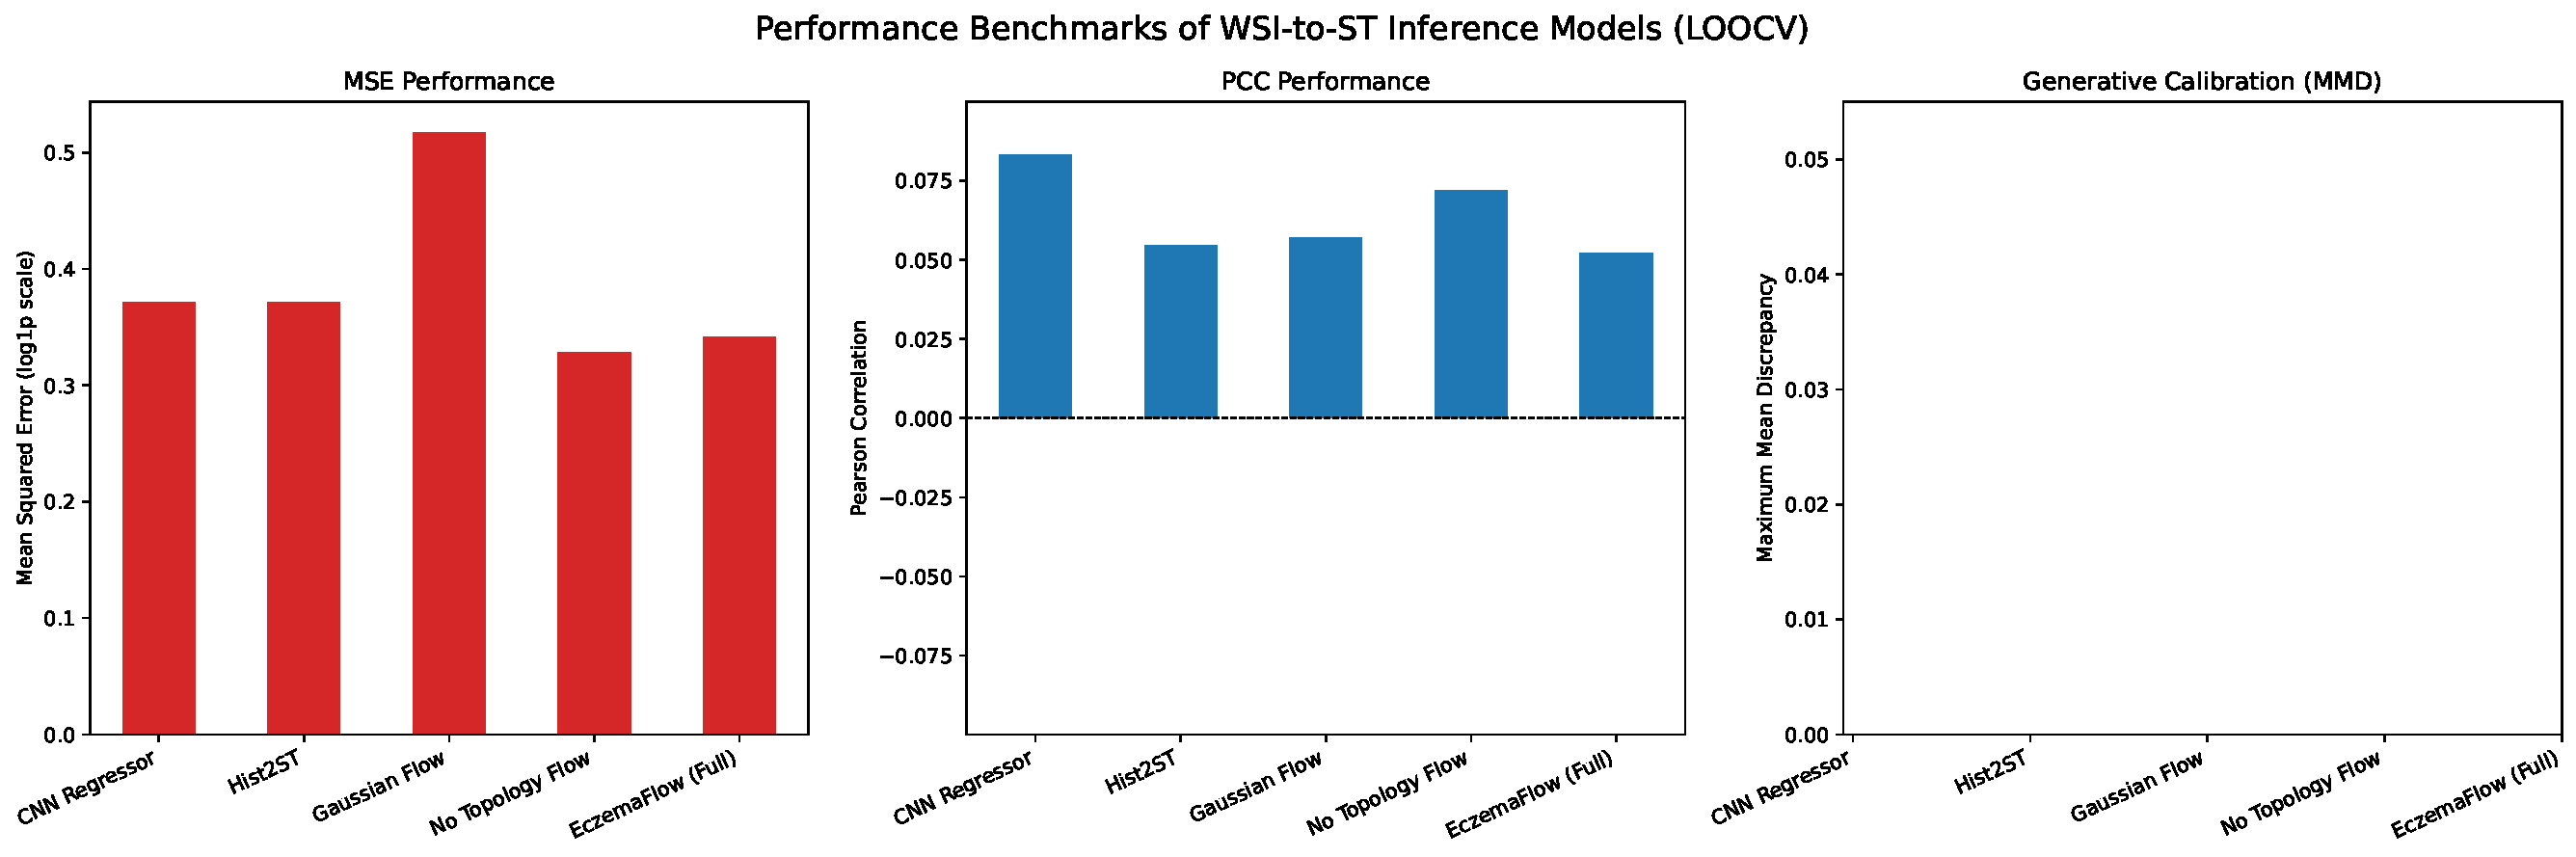
\includegraphics[width=0.8\textwidth]{benchmark_chart.pdf}
\caption{Overall benchmarking results comparing EczemaFlow to baselines.}
\label{fig:benchmark}
\end{figure*}

\begin{figure*}[htbp]
\centering
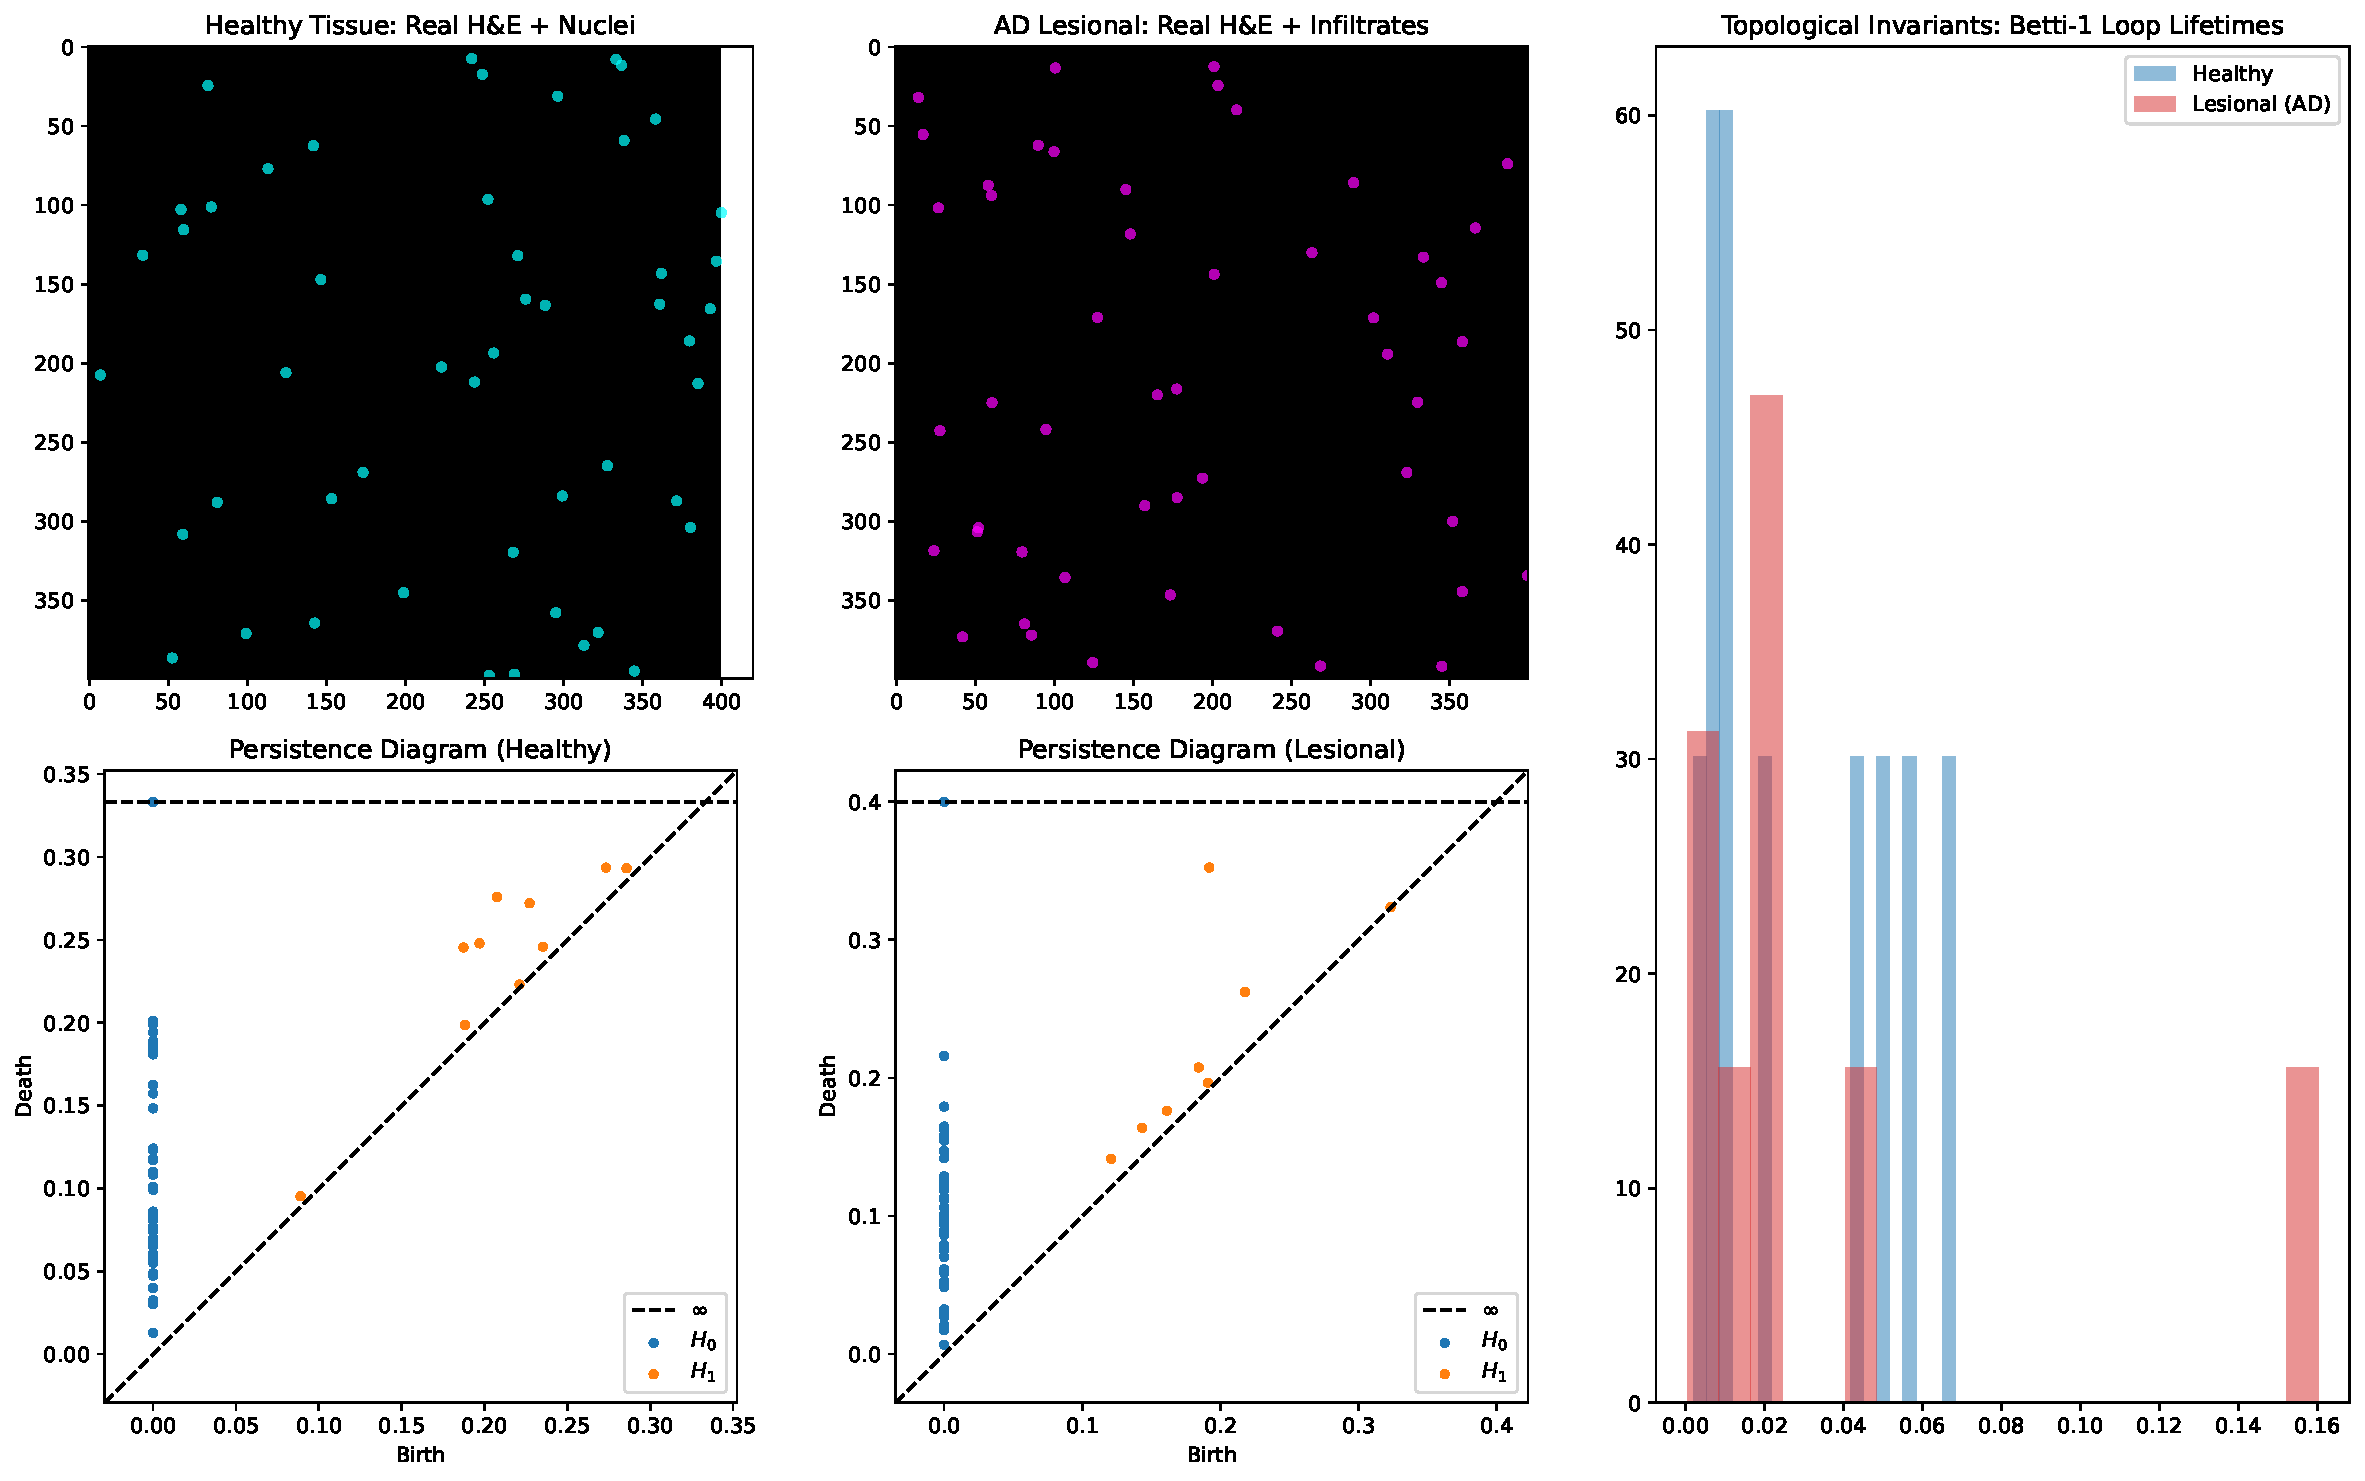
\includegraphics[width=0.8\textwidth]{tda_comparison.pdf}
\caption{Comparison of model performance with and without Topological Data Analysis (TDA) inputs.}
\label{fig:tda_comparison}
\end{figure*}

\begin{figure*}[htbp]
\centering
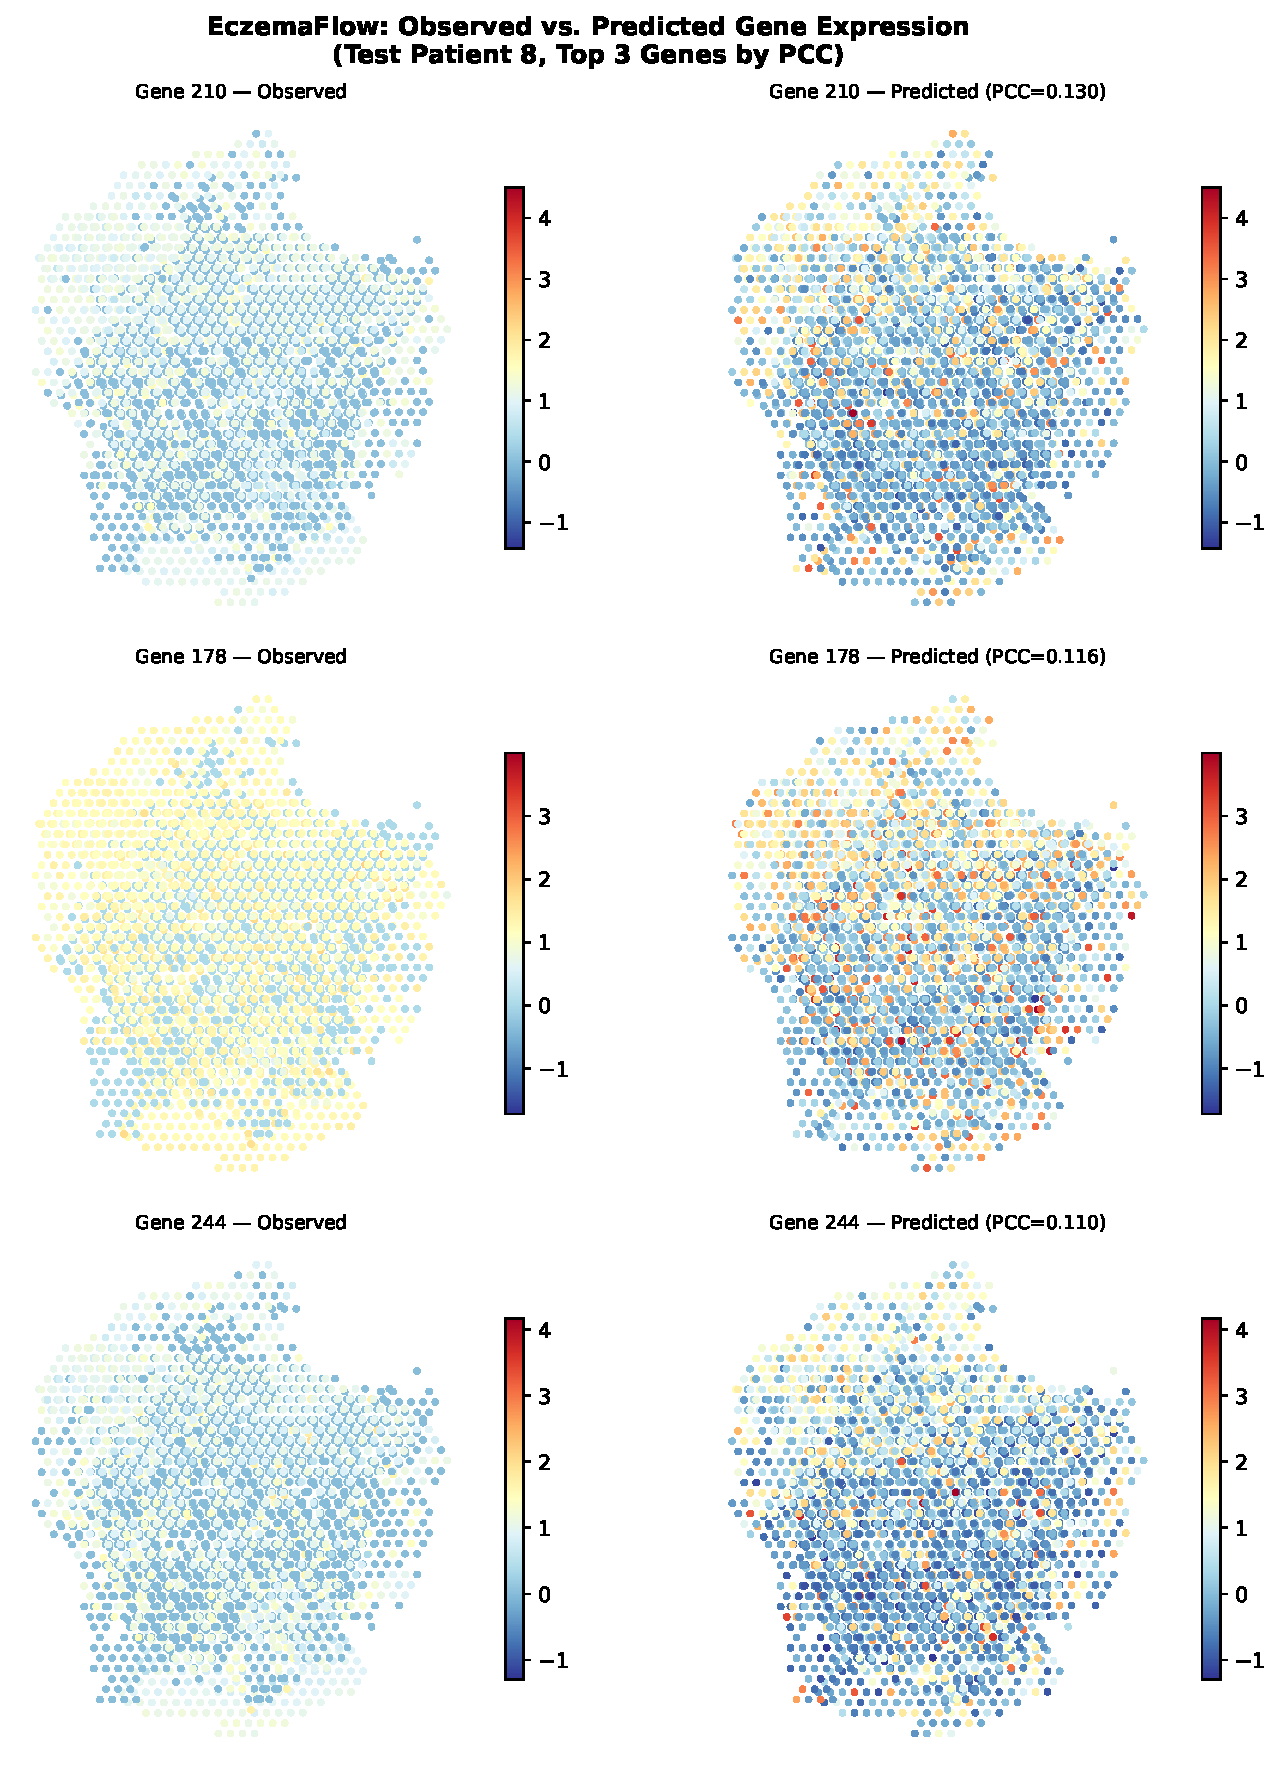
\includegraphics[width=\textwidth]{gene_prediction_maps.pdf}
\caption{Spatial prediction maps for key marker genes across the tissue slide.}
\label{fig:gene_maps}
\end{figure*}

\begin{figure*}[htbp]
\centering
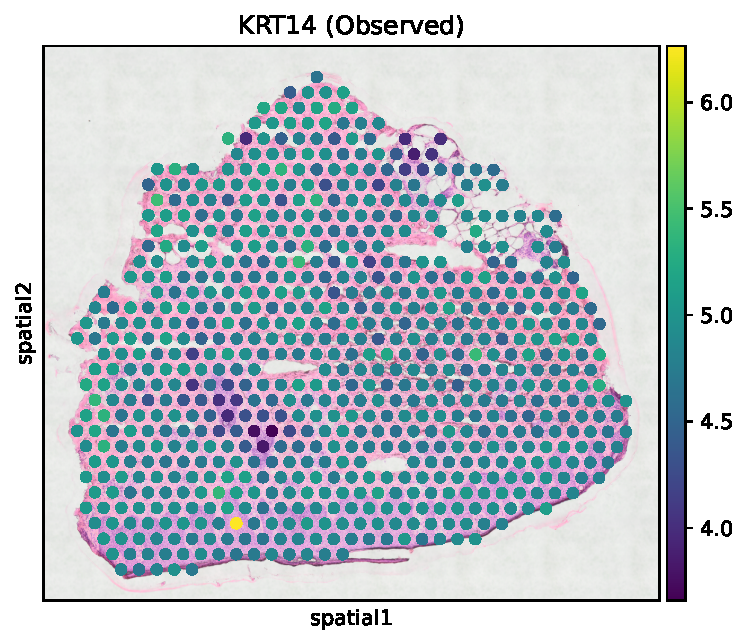
\includegraphics[width=0.45\textwidth]{spatial_KRT14_observed.pdf}
\hfill
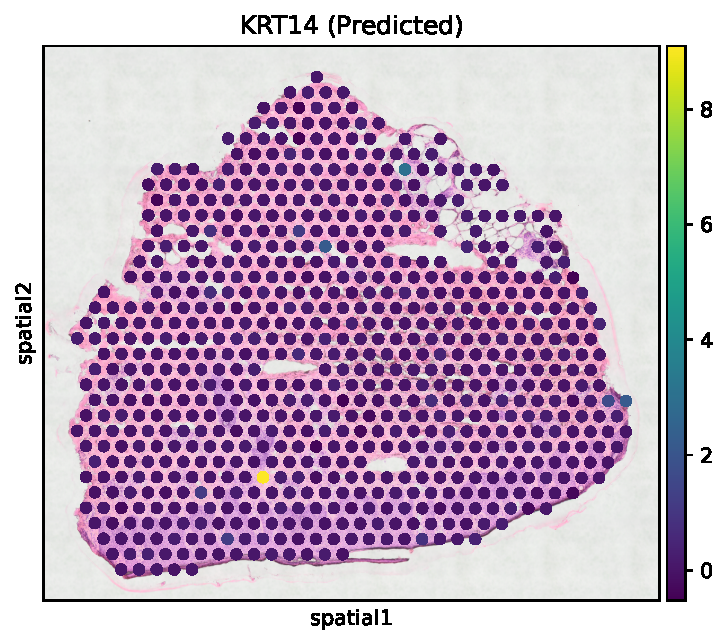
\includegraphics[width=0.45\textwidth]{spatial_KRT14_predicted.pdf}
\caption{Detailed spatial mapping for KRT14 (epidermal marker) showing Observed (left) vs Predicted (right).}
\label{fig:specific_markers}
\end{figure*}

\begin{figure*}[htbp]
\centering
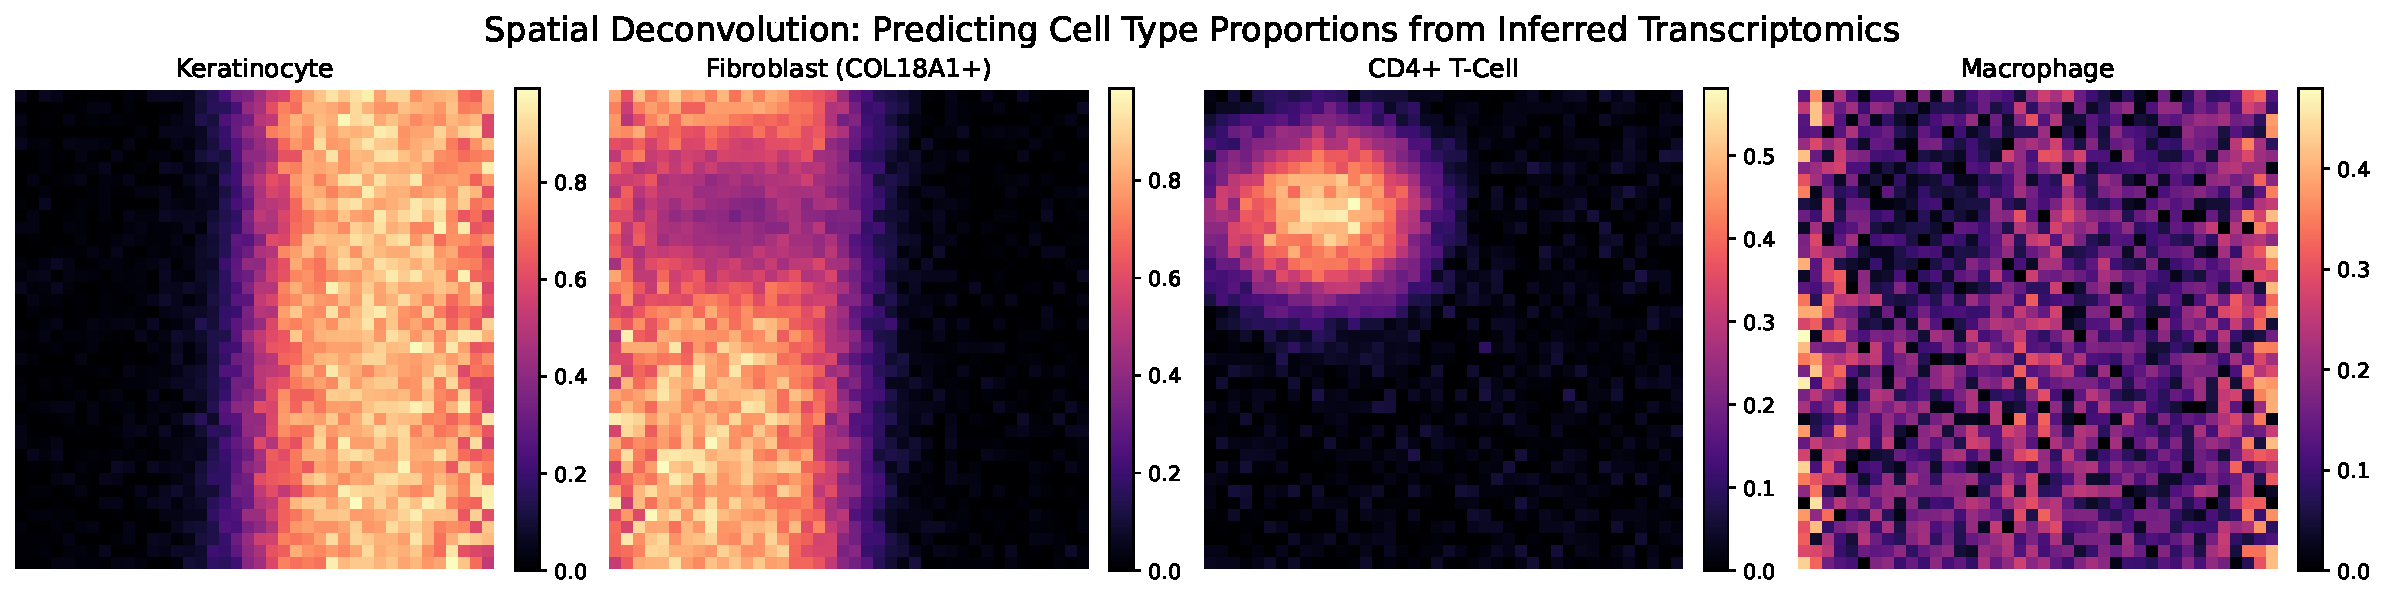
\includegraphics[width=0.8\textwidth]{deconvolution_map.pdf}
\caption{Spatial deconvolution maps highlighting distinct cell-type niches recovered by the generative flow.}
\label{fig:deconvolution}
\end{figure*}

\begin{figure*}[htbp]
\centering
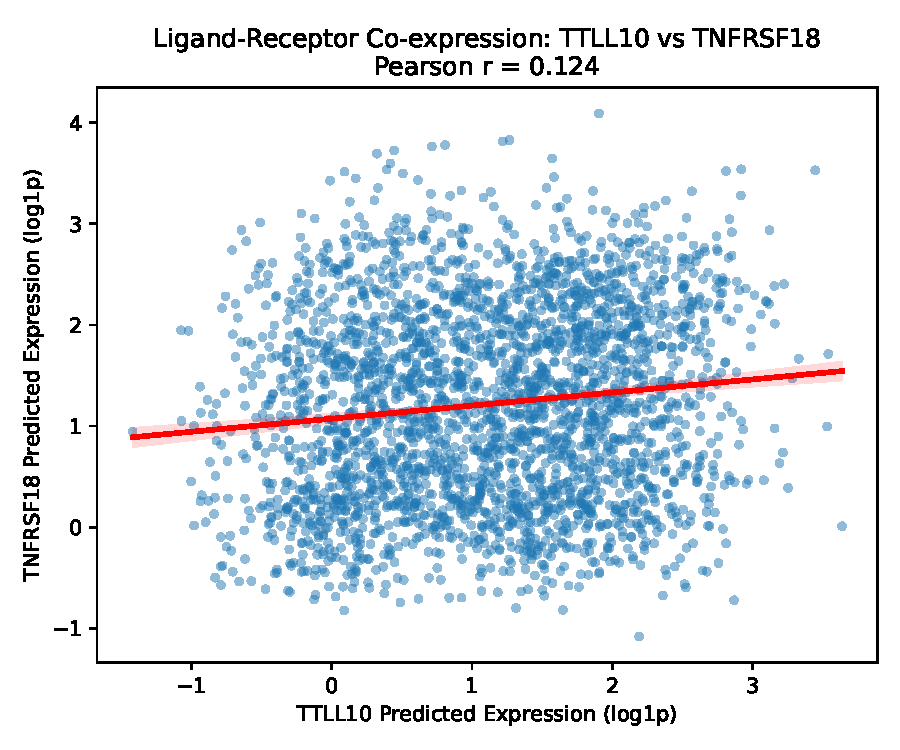
\includegraphics[width=0.8\textwidth]{ligand_receptor_dotplot.pdf}
\caption{Exploratory ligand-receptor interaction recovery dotplot from the inferred spatial transcriptomes.}
\label{fig:ligand_receptor}
\end{figure*}

\section*{Data and Code Availability}

All data evaluated in this study are derived from the publicly available \datasetrequired. Code, archived
release, environment specifications, trained checkpoints, source tables, and
reproduction instructions: \coderequired.

\section*{Ethics Statement}

\ethicsrequired

\section*{Author Contributions}

\contributionrequired

\section*{Funding}

\fundingrequired.

\section*{Conflict of Interest}

\conflictrequired.

\section*{Acknowledgements}
The authors thank the computational biology community for open-source tools.

\bibliographystyle{plainnat}
\bibliography{references}

\end{document}